\tikzstyle{end} = [thin, circle, minimum size = 0.1cm, draw, inner sep = 0.1pt]
\tikzstyle{leaf} = [thin, circle, minimum size = 0.6cm, draw, inner sep = 0.1pt, blue]
\tikzstyle{inner} = [thin, circle, minimum size = 0.2cm, draw, inner sep = 0.1pt, black]
            


\tikzstyle{ed} = [thick, ->, draw, black]

    
\begin{tikzpicture}[black]
    \draw[very thick] (0, 0) rectangle (3, 3);
	\draw[fill = gray!80!white] (0.8, 0.8) rectangle (2.1, 2.2) node[below left] {\scriptsize $R_h$};
    \only<6>{
        \draw[fill = green!20!white, opacity = 0.5, rounded corners] (0.4, 0.4) rectangle (1.4, 2.9) node[below left]
		    {\scriptsize $R_{h'}$};
	    \draw[fill = red!10!white, opacity = 0.5, rounded corners] (1.1, 0.6) rectangle (2.8, 2.5) node[below left]
		    {\scriptsize $R_{h''}$};
    }
    \only<7>{
        \draw[fill = green!20!white, opacity = 0.5, rounded corners] (0.4, 1.2) rectangle (2.8, 2.7) node[below left]
		    {\scriptsize $R_{h'}$};
	    \draw[fill = red!10!white, opacity = 0.5, rounded corners] (0.6, 1.4) rectangle (2.75, 0.5) node[above left]
		    {\scriptsize $R_{h''}$};
    }
\end{tikzpicture}
